\chapter*{Lecture 5}
\begin{recall}{}{}
\begin{itemize}
\item Direct Integration (separable equations)
\item Substitution and Transformation
\end{itemize}
\end{recall}



\section{Exact Equations (corresponds to 2.4 in book)} 
\subsection*{Recall: total and partial derivation}
Let's consider the volume of a cylinder:
\begin{equation*}
V(r,h)=\pi r^{2} h
\end{equation*}
We may be interested to compute the change of volume with regards to the height, $h$ of the cylinder:
\begin{equation*}
\frac{\partial V(r,h)}{\partial h}=\pi r^{2}
\end{equation*}
or, the change of volume with regards to the radius:
\begin{equation*}
\frac{\partial V(r,h)}{\partial r}=2\pi rh
\end{equation*}
%Let's visualize what this means:
%\begin{figure}
%\centering
%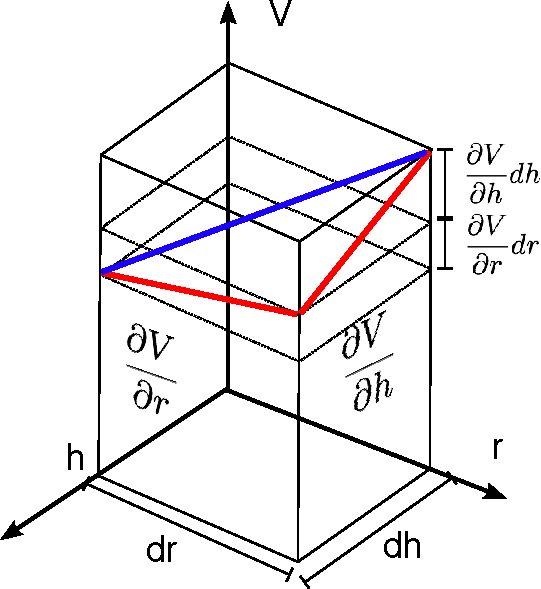
\includegraphics[width=0.5\textwidth]{figs/totalDerivatives.pdf}
%\caption{Change of volume of a cylinder}
%\end{figure}
The \textbf{total derivative}, in some sense, represents the total variation of volume $V$.
\begin{equation*}
dV=\frac{\partial V}{\partial h} dh+\frac{\partial V}{\partial r} dr
\end{equation*}

\begin{exmp}{Total derivative:}
Suppose,
\begin{equation*}
f(x,y)=3x^{2}y+5xy+y^{3}+5
\end{equation*}
Then the differential of $f(x,y)$ would be:
\begin{equation*}
df=\frac{\partial f(x,y)}{\partial x} dx+\frac{\partial f(x,y)}{\partial y} dy
\end{equation*}
where:
\begin{equation*}
\frac{\partial f(x,y)}{\partial x} = (6xy+5y)
\end{equation*}
and
\begin{equation*}
\frac{\partial f(x,y)}{\partial y}=3x^{2}+5x+3y^{2}
\end{equation*}
The \textbf{total differential} would be:
\begin{equation*}
df= (6xy+5y)dx+(3x^{2}+5x+3y^{2})dy \qquad \bLozenge
\end{equation*}
\end{exmp}

Now, what if we are asked to solve the following differential expression?
\begin{equation*}
(6xy+5y)dx+(3x^{2}+5x+3y^{2})dy=0
\end{equation*}
It would be clear from the previous example (if and only if, it satisfies the properties of a total derivative), that we would simply need to solve the total differential of a function $f(x,y)$ when $df=0$!\\



\begin{defin}{Exact equation}{}
A differential expression :
 \begin{equation*}
M(x,y) dx+N(x,y)dy
\end{equation*}
is called an \textbf{exact equation} if it is the total differential of a function $F(x,y)$, i.e. if:
 \begin{equation*}
M(x,y) =\frac{\partial F(x,y)}{\partial x} \qquad \text{and} \qquad N(x,y) =\frac{\partial F(x,y)}{\partial y}
\end{equation*}
\end{defin}


\begin{defin}{Compatibility condition}{}
Consider an exact equation which can be written as:
 \begin{equation*}
M(x,y) dx+N(x,y)dy=\frac{\partial F}{\partial x}dx+\frac{\partial F}{\partial y}dy
\end{equation*}
We recall the continuous partial derivatives we may swap the order of the derivative operator:
\begin{equation*}
\frac{\partial}{\partial y}\frac{\partial F}{\partial x}=\frac{\partial}{\partial x}\frac{\partial F}{\partial y}
\end{equation*}
As a result, the compatibility condition would dictate that:
\begin{equation*}
\boxed{\frac{\partial}{\partial y}M(x,y)=\frac{\partial}{\partial x}N(x,y)}
\end{equation*}
\end{defin}




\subsection{Solving for exact equations}
\begin{enumerate}
\item Reformulate the first-order ODE as $Mdx+Ndy=0$
\item Check exactness of equation (compatibility condition): $\frac{\partial}{\partial y}M(x,y)=\frac{\partial}{\partial x}N(x,y)$
\item Find $F(x,y)$ with the relation: $F(x,y)=\int Mdx+g(y)$
\item Determine $g(y)$ by solving: $\partial F(x,y)/\partial y = N$
\item Set (and, if possible, determine) $C$
\end{enumerate}

\begin{center}
\noindent\rule{4cm}{0.4pt}
\end{center}

\begin{exmp}{}
Solve the differential equation of the form:
\begin{equation*}
\frac{dy}{dx}=-\frac{2xy^{2}+1}{2x^{2}y}
\end{equation*}
Can we solve by direct integration ? Substitution? Not obvious. Let's try see if we can rewrite the equation.

\textbf{Solution:}
\begin{enumerate}

\item   Re-write as:
\begin{equation*}
({2xy^{2}+1})dx+(2x^{2}y)dy=0
\end{equation*}

where $M(x,y)={2xy^{2}+1}$ and $N(x,y)=2x^{2}y$.
\item Let's see if the equation is exact. We check the compatibility condition:
\begin{equation*}
\frac{\partial}{\partial y}M(x,y)= 4xy \qquad
\frac{\partial}{\partial x}N(x,y)=4xy
\end{equation*}
We have an exact equation!

\item Let's try to find the function that is the total derivative of the equation:
\begin{equation*}
\frac{\partial}{\partial x} F(x,y)=M(x,y)
\end{equation*}
\begin{equation*}
F(x,y)=\int M(x,y) dx + g(y)=\int ({2xy^{2}+1})dx +g(y)=x^2y^2+x+g(y)
\end{equation*}
Note that $g(y)$ represents the integration constant. Since it emerged from an integration with regards to $x$, the integrative constant can, in the most general sense, be a function of $y$. (derive the above eq with regards to $x$ to verify)
\item  Let's find $g(y)$ by deriving the function $F(x,y)$ with regards to $y$:
\begin{equation*}
\frac{\partial F(x,y)}{\partial y}= N(x,y)= 2x^2y+g'(y)
\end{equation*}
The LHS must be equal to $N$, therefore $g'(y)=0$ or $g=c$
\item The final solution is:
\begin{equation*}
\boxed{F(x,y)=x^2y^2+x+c}
\end{equation*}
(the problem did not specify an IC)
\end{enumerate}
\end{exmp}

\begin{center}
\noindent\rule{4cm}{0.4pt}
\end{center}
\updateinfo[September 19, 2018]

